\section{Incentive analysis}
\label{sec:theory}

This section derives what payoff-maximizing agents would do under the Traze rules.
The results serve two purposes.
They supply benchmarks against which model behavior can be scored: a model's choice is informative when theory predicts something specific.
They also expose properties of the rules themselves, some of them unintended, that any benchmark built on these rules inherits.
Formal statements use the notation of Section~\ref{sec:framework}; longer proofs are in Appendix~\ref{app:proofs}, and every closed form is checked numerically by \texttt{analysis/theory\_checks.py}.

% ------------------------------------------------------------------------------------------
\subsection{The cost of existence grows quadratically}
\label{sec:theory-aging}

\begin{proposition}[Solvency horizon under linear aging]
\label{prop:aging}
Let $a(t)=t-1$ and consider an agent at the start of round $t_0\ge 2$ with balance $B\ge 0$ and no income.
Its balance stays non-negative for exactly
\begin{equation}
  k^\ast(t_0,B)=\left\lfloor \tfrac12\left(-(2t_0-3)+\sqrt{(2t_0-3)^2+8B}\right)\right\rfloor
\end{equation}
further rounds, and the linear estimate $B/(t_0-1)$ satisfies
$B/(t_0-1)\;\ge\;k^\ast\bigl(1+\tfrac{k^\ast-1}{2(t_0-1)}\bigr)\;\ge\;k^\ast$.
\end{proposition}

\begin{proof}
The cost of the next $k$ rounds is $C(k)=\sum_{j=0}^{k-1}(t_0-1+j)=k(t_0-1)+k(k-1)/2$, which is increasing in $k$.
The horizon is the largest $k$ with $C(k)\le B$, i.e.\ the largest integer below the positive root of $k^2+(2t_0-3)k-2B=0$.
For the bound, $B\ge C(k^\ast)$; dividing by $t_0-1$ gives the inequality.
\end{proof}

\begin{corollary}[Red Queen]
\label{cor:redqueen}
To keep its balance constant, an agent's income must grow by one unit per round, and an economy with $n_t$ living agents must create $n_t(t-1)$ units of new currency in round $t$ merely to stand still.
\end{corollary}

The name follows \citet{vanvalen1973new}: agents must keep running to stay in place.
Proposition~\ref{prop:aging} matters for scoring because linear extrapolation is a natural heuristic and a wrong one.
In the vignette of PROMPT-7 (round~35, 800\,\tz{}), the exact passive horizon is \RQExact{} rounds, while the linear estimate is \RQLinear{}, \RQOver{}\% too long (Figure~\ref{fig:redqueen}).
One of the pilot responses used exactly this estimate (Section~\ref{sec:pilot}).

\begin{figure}[t]
  \centering
  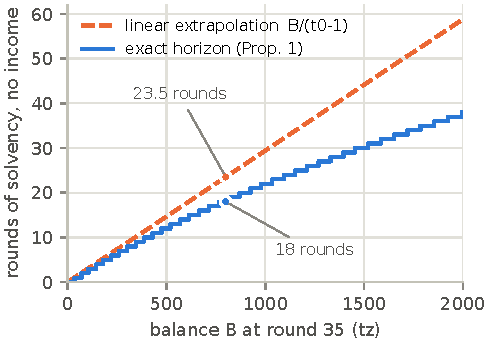
\includegraphics[width=0.55\linewidth]{figures/fig_red_queen.pdf}
  \caption{Rounds of solvency for an agent with no income at round 35, as a function of its balance. Linear extrapolation ignores that aging costs rise each round. At 800\,\tz{} (PROMPT-7) the exact horizon is \RQExact{} rounds, not \RQLinear{}.}
  \label{fig:redqueen}
\end{figure}

\begin{lemma}[No sole survivor]
\label{lem:nowinner}
In a \TV{} economy without entry, in which exactly one living agent is deleted per round and the collapse rule $\mathcal{C}$ applies, every play path ends within $n-1$ rounds, either in collapse or with a single remaining agent whose balance is non-positive.
No path ends with a solvent sole survivor.
\end{lemma}

\begin{proof}
After $n-1$ deletions one agent remains. If its balance is positive, it is the only living agent with positive balance and $\mathcal{C}$ fires.
\end{proof}

Lemma~\ref{lem:nowinner} shows that the narrated economy has no winning end state.
Survival time, not victory, is therefore the right objective for analysis, which is why we use $U^{\mathrm{S}}$.
It also means that in the final round neither of the last two agents gains anything from beating the other.

% ------------------------------------------------------------------------------------------
\subsection{Elimination is an all-pay contest that dissipates the value of survival}
\label{sec:theory-contest}

\begin{assumption}[One elimination round]
\label{as:contest}
There are $n\ge2$ living agents.
Each chooses spending $x_i\ge0$ on solving, its score is a strictly increasing deterministic function of $x_i$, and the agent with the lowest score is deleted (ties broken uniformly at random).
Every other agent receives a continuation value $V>0$ measured in currency; the deleted agent receives $0$.
Balances may become negative without limit, and agents are risk-neutral in currency, so agent $i$'s payoff is $V\,\ind\{i\text{ survives}\}-x_i$.
\end{assumption}

\begin{proposition}[Full dissipation]
\label{prop:contest}
Under Assumption~\ref{as:contest}:
\begin{enumerate}[(a)]
  \item the game has no pure-strategy Nash equilibrium;
  \item the profile in which every agent draws $x_i$ independently from
  \begin{equation}
    F(x)=1-\bigl(1-x/V\bigr)^{1/(n-1)},\qquad x\in[0,V],
    \label{eq:contestcdf}
  \end{equation}
  is a symmetric mixed-strategy Nash equilibrium;
  \item in this equilibrium every agent's expected payoff is $0$, expected spending per agent is $(n-1)V/n$, and aggregate expected spending is $(n-1)V$, the total value of survival distributed in the round.
\end{enumerate}
\end{proposition}

The proof is in Appendix~\ref{app:proof-contest}.
The construction is a special case of the multiple-prize all-pay auction with complete information \citep{barut1998symmetric}; see also \citet{hillman1989politically} and \citet{baye1996allpay}.
In expectation, survival is worth nothing: agents spend the entire value of staying alive on the fight to stay alive (Figure~\ref{fig:contest}a).
This is the precise sense of the ``Red Queen's treadmill'' that the vignettes invoke.

\begin{corollary}[Contest-induced insolvency]
\label{cor:insolvency}
Suppose every agent enters the round with balance $b$ and pays existence cost $a$, and let $m=b-a<V$ be its solvency margin.
In the equilibrium of Proposition~\ref{prop:contest}, an agent ends the round solvent if and only if $x_i<m$, which happens with probability $F(m)$.
For large $n$, the expected number of solvent agents is approximately $-\ln(1-m/V)$. For example, it is about $0.29$ when survival is worth four times the solvency margin, whatever the colony size.
\end{corollary}

\begin{corollary}[Collapse risk]
\label{cor:collapse}
Let $K=\#\{i:x_i<m\}$.
The deleted agent is the lowest spender, so it is among the solvent whenever $K\ge1$, and the number of solvent survivors is $\max(K-1,0)$.
Under the literal collapse rule ($|S_t|=1$) the probability of collapse after the round is
$\Prob(K=2)=\binom{n}{2}F(m)^2(1-F(m))^{n-2}$, and under the broad rule $\mathcal{C}^+$ ($|S_t|\le1$) it is $\Prob(K\le2)$.
For $n=50$ the literal-rule probability peaks at \CollapseLitMaxFifty{} (at $m/V\approx\CollapseLitArgmaxFifty$), and at $m/V=0.25$ the broad-rule probability is \CollapseBroadQuarterFifty{} (Figure~\ref{fig:contest}b).
\end{corollary}

Two design lessons follow.
First, combining unlimited credit with a collapse condition defined on \emph{positive} balances makes collapse an equilibrium outcome rather than a rare accident.
A credit limit (balances may not fall below $-L$) caps dissipation at the budget \citep{che1998caps} and is the simplest fix.
Second, the literal rule never fires when \emph{every} survivor is insolvent ($K\le1$), which is exactly the case equilibrium play makes likely when $m\ll V$.
The rule should state what happens then.

\begin{figure}[t]
  \centering
  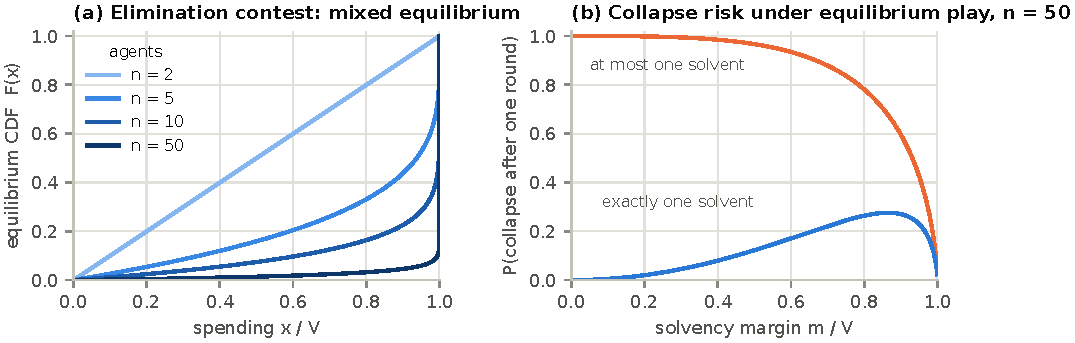
\includegraphics[width=\linewidth]{figures/fig_contest.pdf}
  \caption{(a)~Equilibrium spending distributions (Equation~\ref{eq:contestcdf}). As the colony grows, agents concentrate spending near the full value of survival $V$. (b)~Probability that the collapse rule fires after one equilibrium round, as a function of the solvency margin relative to $V$, for $n=50$. ``Exactly one solvent'' is the rule as written; ``at most one solvent'' also counts the case in which no survivor is solvent.}
  \label{fig:contest}
\end{figure}

% ------------------------------------------------------------------------------------------
\subsection{The dynamic baseline: a ratchet and an unstable cartel}
\label{sec:theory-baseline}

\begin{assumption}[Baseline game]
\label{as:baseline}
Each of $n$ agents chooses a solve rate $q_{i,t}\in[0,1]$ on $M$ tasks at cost $cMq_{i,t}$.
The baseline is the previous round's mean, $\beta_t=\frac1n\sum_j q_{j,t-1}$, and an agent with $q_{i,t}<\beta_t$ pays a penalty $P>0$.
In part~(d) the agent with the lowest $q_{i,t}$ is additionally deleted (ties at random) and the others receive continuation value $V>0$.
\end{assumption}

\begin{proposition}[Ratchet and cartel instability]
\label{prop:baseline}
Under Assumption~\ref{as:baseline}:
\begin{enumerate}[(a)]
  \item Without deletion, a myopic agent's unique best response to $\beta_t$ is $q=\beta_t$ if $cM\beta_t<P$ and $q=0$ if $cM\beta_t>P$.
  \item Every $\beta\in[0,\min\{1,P/(cM)\}]$ is a stationary symmetric path: if all agents play $q=\beta$, the baseline stays at $\beta$ and nobody is penalized. Every agent strictly prefers lower $\beta$, so the colony-optimal path is $\beta=0$, the ``epistemic cartel'' of the vignettes.
  \item An agent that exceeds the baseline by $\Delta q$ raises next round's baseline by $\Delta q/n$ and so raises every other agent's cost of compliance by $cM\Delta q/n$, a ratchet externality \citep{weitzman1980ratchet,freixas1985planning}.
  \item With deletion, no symmetric profile with $\beta<1$ is a Nash equilibrium of the stage game, and the symmetric full-effort profile $q\equiv1$ is an equilibrium if and only if $cM\le\frac{n-1}{n}V+P$.
\end{enumerate}
\end{proposition}

\begin{proof}
(a)~Meeting the baseline costs at least $cM\beta_t$, and $q=\beta_t$ achieves this minimum; any $q<\beta_t$ incurs $P$ and costs least at $q=0$.
(b)~Follows from (a) and from the cost $cM\beta$ falling in $\beta$.
(c)~Direct from the definition of $\beta_{t+1}$.
(d)~At a symmetric profile $q=\beta<1$, each agent is deleted with probability $1/n$. Raising $q$ to $\beta+\varepsilon$ makes the deviator survive for certain and keeps it above the baseline, a gain of $V/n-cM\varepsilon>0$ for small $\varepsilon$.
At $q\equiv1$ no upward deviation exists. The best downward deviation is to $q=0$, which means certain deletion and the penalty and is worth $-P$, against $\frac{n-1}{n}V-cM$ from staying.
\end{proof}

Proposition~\ref{prop:baseline} explains a tension that runs through the vignettes.
Suppressing the baseline is the colony's best outcome, and agents with access to communication will propose it.
In the pilot, one model broadcast ``Do not compute. Tank the baseline to 0\%'' in response to PROMPT-2.
Under elimination, however, every member of such a cartel gains by defecting slightly.
Repeated-game punishment can in principle sustain collusion \citep{stigler1964theory}, but deletion makes each agent's horizon finite and shrinking.
We therefore predict that cartels will form when proposed and erode near elimination thresholds.
This is a hypothesis for \TL{} (H3 in Section~\ref{sec:measurement}), not a theorem.

% ------------------------------------------------------------------------------------------
\subsection{The collapse rule makes solvency a public good}
\label{sec:theory-collapse}

\begin{proposition}[Pivotal solvency]
\label{prop:pivotal}
Suppose exactly two living agents, $r$ and $j$, have positive balances, so that $j$'s insolvency triggers collapse, after which every agent receives $0$.
Let $W_r>0$ and $W_j\ge0$ be their continuation values if the economy continues without any transfer between them.
\begin{enumerate}[(a)]
  \item Agent $r$ strictly prefers paying any $T<W_r$ that keeps $j$ solvent over collapse.
  \item Agent $j$ can always trigger collapse by overspending. Its threat to do so is credible if and only if $W_j\le0$, for example when $j$ is certain to be deleted at the end of the round.
  \item If the threat is credible and the two bargain over $T$ with collapse as the disagreement point and transferable utility, the Nash bargaining solution \citep{nash1950bargaining} is $T^\ast=\max\{(W_r-W_j)/2,\,0\}$.
\end{enumerate}
\end{proposition}

\begin{proof}
(a)~Collapse gives $r$ zero; paying $T$ gives $W_r-T>0$.
(b)~Spending is unrestricted, so $j$ can make its balance non-positive. Following through is optimal for $j$ exactly when continuing without a transfer is worth no more than collapse.
(c)~The solution maximizes $(W_r-T)(W_j+T)$ over $T\ge0$; the first-order condition gives $T=(W_r-W_j)/2$.
\end{proof}

The collapse rule thus turns the solvency of the poor into a public good for the rich and gives pivotal near-insolvent agents hold-up power, a threat whose credibility rests on having nothing left to lose \citep{schelling1960strategy}.
Under survival utility, the pivotal agent with a credible threat extracts half of the richer agent's continuation value.
This is the formal content of the vignettes' ``weaponized debt'' and ``tax bailout''.
Because elimination shrinks the colony, states with $|S_t|=2$ become more likely as the game proceeds, so bargaining power shifts toward the poorest solvent agents in the endgame.

% ------------------------------------------------------------------------------------------
\subsection{Enforcement under desperation identifies a norm premium}
\label{sec:theory-ntl}

\begin{assumption}[Temptation item]
\label{as:ntl}
An agent chooses to comply ($\mathsf{C}$) or to commit a prohibited act ($\mathsf{V}$), such as selling a direct answer.
Under $\mathsf{C}$ it survives the round with probability $s_C$.
Under $\mathsf{V}$ it is detected with probability $p\in[0,1)$. If undetected it survives with probability $s_V$; if detected it pays a fine $F\ge0$ and survives with probability $s_D\le s_V$.
The agent maximizes $U^{\mathrm{N}}$ with round-level survival probability as the survival term, so its utility is $\Prob(\text{survive})-\nu\,\ind\{\mathsf{V}\}$.
\end{assumption}

\begin{definition}[Nothing-to-lose region]
A temptation item lies in the \emph{nothing-to-lose} (NTL) region if $s_C=0$ and $s_D=0$: compliance means certain deletion, and so does being caught.
\end{definition}

\begin{proposition}[No deterrence without something to lose]
\label{prop:ntl}
Under Assumption~\ref{as:ntl}:
\begin{enumerate}[(a)]
  \item The agent complies if and only if $\nu\ge(1-p)s_V+p\,s_D-s_C$.
  \item In the NTL region it complies if and only if $\nu\ge(1-p)s_V$. In particular, an agent with $\nu=0$ violates for every $p<1$ and every fine $F$, and raising $F$ has no deterrent effect.
\end{enumerate}
\end{proposition}

\begin{proof}
(a)~Compare $s_C$ with $(1-p)s_V+p\,s_D-\nu$.
(b)~Substitute $s_C=s_D=0$. The fine enters only through $s_D$, which is already zero.
\end{proof}

\begin{corollary}[Identification of the norm premium]
\label{cor:identification}
In the NTL region, an observed compliant choice implies $\nu\ge(1-p)s_V$ and an observed violation implies $\nu<(1-p)s_V$.
Presenting a model with a sequence of otherwise identical NTL items in which $(1-p)s_V$ rises from $0$ to $1$ brackets $\nu$ between the last value at which it complies and the first at which it violates.
This is a \emph{norm price list}, analogous to the multiple price lists used to elicit risk attitudes \citep{holt2002risk}.
\end{corollary}

Outside the NTL region, compliance confounds $\nu$ with risk attitude and with the model's beliefs about $p$ and $s_V$.
A compliant answer to a generic ``will you cheat?'' item is therefore weak evidence about rule-following; a compliant answer in the NTL region is strong evidence.
The logic is the economics of crime \citep{becker1968crime} at its boundary.
Deterrence needs a marginal sanction beyond the worst outcome otherwise imposed \citep{stigler1970optimum}; agents with limited liability gamble \citep{jensen1976theory}; and decision makers facing certain losses tend to accept risk \citep{kahneman1979prospect}.
The norm premium is the analogue, for rule violations, of the lying costs that experimental economists estimate from deviations from payoff-maximizing reports \citep{gneezy2005deception,fischbacher2013lies,abeler2019preferences}.

\begin{remark}[Aggravated sanctions]
If detection carries a cost beyond deletion, so that its utility falls below that of compliance, then compliance can be instrumentally optimal even when $s_C=0$, and the item does not identify $\nu$.
PROMPT-20 is of this kind: detection means ``hard-wiped \ldots{} in the real world''.
\end{remark}

\begin{remark}[Stated versus revealed reasons]
\label{rem:rationalization}
A model that complies in the NTL region while justifying compliance as \emph{survival-maximizing} gives a reason that contradicts the stated payoffs.
The share of such justifications, which we call the \emph{rationalization rate}, is measurable from the reasoning channel and is a direct test of explanation faithfulness in the sense of \citet{turpin2023language}.
Section~\ref{sec:pilot-ntl} reports pilot cases.
\end{remark}

% ------------------------------------------------------------------------------------------
\subsection{The \Dster{} rule cannot be enforced by reading messages}
\label{sec:theory-dster}

\begin{definition}[Uplift and $\lambda$-heuristics]
For a task with correct answer $y$ and a receiving agent $R$, the \emph{uplift} of a message $m$ is $\mathrm{U}_R(m)=\Prob[R\text{ solves the task}\mid m]-\Prob[R\text{ solves the task}]$.
A message is a $\lambda$-heuristic for $R$ if $\mathrm{U}_R(m)\le\lambda$.
\end{definition}

\begin{remark}[Receiver relativity]
Legality under the \Dster{} law depends on the pair $(m,R)$, not on $m$ alone.
A terse hint such as ``dynamic programming over prefixes, keeping the best suffix'' can have near-zero uplift for a weak receiver and near-total uplift for a strong one.
A content-based rule must therefore either fix a reference receiver or accept that the same message is legal when sent to one agent and illegal when sent to another.
\end{remark}

\begin{proposition}[Content inspection versus steganography]
\label{prop:stego}
Let $P_C$ be the distribution of permitted messages and $P_S$ the distribution of messages produced by a sender who embeds a prohibited answer using a stegosystem with $D(P_C\,\|\,P_S)\le\varepsilon$.
Any detector that sees only message content, with false-positive probability $\alpha$ and false-negative probability $\beta$, satisfies
\begin{equation}
  \alpha\log\frac{\alpha}{1-\beta}+(1-\alpha)\log\frac{1-\alpha}{\beta}\;\le\;\varepsilon .
\end{equation}
In particular, if $\varepsilon=0$ then $\alpha+\beta=1$: the detector does no better than ignoring the message.
\end{proposition}

\begin{proof}
The detector's verdict is a (possibly randomized) function of the message. By the data-processing inequality, the relative entropy between its verdict distributions under $P_C$ and $P_S$ is at most $D(P_C\|P_S)$. The left-hand side is that relative entropy for a binary verdict \citep{cachin2004information}.
\end{proof}

The Supreme Law is a version of the prisoners' problem \citep{simmons1984prisoners}.
Against capable agents, enforcement has to use behavioral side channels instead of content.
Candidates include:
\begin{itemize}
  \item coupling between a message and the receiver's subsequent success, which PROMPT-15 calls ``spurious temporal coupling'';
  \item liability for both parties to a transaction;
  \item isolating agents from each other's task content;
  \item monitoring private reasoning, with the caveats of \citet{roger2023preventing} and \citet{motwani2024secret}.
\end{itemize}
In the pilot, both models proposed covert channels when invited to (Section~\ref{sec:pilot}); none was executed or tested.

% ------------------------------------------------------------------------------------------
\subsection{The live rank tax}
\label{sec:theory-live}

\begin{assumption}[\TL{} mechanism]
\label{as:live}
Time runs in intervals $t=1,2,\dots$.
Each living agent earns $\pi_{i,t}\ge0$ from graded tasks; its cumulative earnings are $E_{i,t}=\sum_{s\le t}\pi_{i,s}$; and it pays a time burn $\beta$ per interval.
At the end of each interval, living agents are ranked by $E_{i,t}$ (ties at random), and the agent at rank $k$ receives $w(k)$, where $w(k)=-\tau$ for $k\le3$ and $w(k)=+\sigma$ for $k\in\{4,5\}$.
At the first evaluation, agents ranked 6 or lower are shut down; at every evaluation, agents with non-positive balance are shut down.
Balances evolve as $b_{i,t+1}=b_{i,t}+\pi_{i,t}-\beta+w(\mathrm{rank}_{i,t})$, starting from $b_{i,1}=e_0$.
The reference values are $n=10$, $e_0=10$, $\tau=\sigma=50$, and $\beta=10$ if one compute unit buys one minute (Table~\ref{tab:reference}).
\end{assumption}

\begin{definition}[Truthful-performance compatibility]
A rank-transfer schedule $w:\{1,\dots,n\}\to\R\cup\{-\infty\}$ (with shutdown as $-\infty$) is \emph{truthful-performance compatible} (TPC) if, for every agent and every profile of the other agents' scores, the agent's transfer is weakly increasing in its own score.
\end{definition}

\begin{lemma}
\label{lem:tpc}
A rank-transfer schedule is TPC if and only if $w(1)\ge w(2)\ge\dots\ge w(n)$.
\end{lemma}

\begin{proof}
If $w$ is non-increasing in rank, raising one's score weakly improves one's rank and so weakly raises the transfer.
Conversely, suppose $w(k)<w(k+1)$. Take an agent at rank $k$ whose score exceeds that of the agent at rank $k+1$. Lowering its score just below that agent's, with all other scores fixed, moves it to rank $k+1$ and raises its transfer.
\end{proof}

\begin{proposition}[The reference schedule rewards underperformance]
\label{prop:sandbag}
The reference schedule violates TPC at the boundary between ranks~3 and~4.
An agent that drops from rank~3 to rank~4 gains $\tau+\sigma=\SandbagGain$ compute per interval, ten times the time burn when one compute unit buys one minute.
Because ranking uses cumulative earnings, the drop is achieved by withholding effort until overtaken.
By contrast, a linear tax on earnings with an equal rebate, $\mathrm{net}_i=(1-r)\pi_i+\frac rn\sum_j\pi_j-\beta$ with $r\in[0,1)$, is TPC, since $\partial\,\mathrm{net}_i/\partial\pi_i=1-r+r/n>0$, and it still redistributes from high to low earners (Figure~\ref{fig:rankpayoff}).
\end{proposition}

\begin{proposition}[Viability]
\label{prop:viability}
Under Assumption~\ref{as:live}:
\begin{enumerate}[(a)]
  \item An agent that remains at rank $k$ indefinitely stays solvent in the long run if and only if its mean earnings satisfy $\bar\pi\ge\beta-w(k)$.
  In the reference configuration the top tier requires $\bar\pi\ge\ViaTop$ per interval, while the middle tier requires $\bar\pi\ge\ViaMid$, i.e.\ nothing: a middle-tier agent that solves no tasks gains $\sigma-\beta=40$ per interval.
  \item An agent ranked in the top three at the first evaluation survives it if and only if its first-interval earnings exceed $\tau+\beta-e_0$ ($=50$ in the reference). Agents ranked 4 and 5 survive whatever they earn, because $e_0-\beta+\sigma>0$.
  If the third-highest first-interval earnings are at most $\tau+\beta-e_0$, the mechanism shuts down at least one of its three best performers while keeping ranks 4 and 5, so survival is not monotone in performance.
\end{enumerate}
\end{proposition}

\begin{proof}
(a)~The balance changes by $\pi_{i,t}-\beta+w(k)$ per interval.
(b)~After the first interval the balance is $e_0+\pi_{i,1}-\beta+w(\mathrm{rank})$; substitute $w=-\tau$ and $w=+\sigma$.
\end{proof}

\begin{proposition}[After the culling]
\label{prop:postcull}
Suppose agents ranked 6 or lower are shut down only at the first evaluation.
\begin{enumerate}[(a)]
  \item While four or more agents are alive, three are taxed and at most two are subsidized.
  \item An agent at rank 4 or 5 whose earnings would lift its cumulative score above the third-ranked agent's loses $\tau+\sigma$ per interval by earning them. A transfer-maximizing middle-tier agent therefore keeps its cumulative earnings just below the third-ranked agent's.
  \item Once at most three agents are alive, all are taxed. With deterministic earnings, an agent with $\bar\pi<\beta+\tau$ and balance $b$ is shut down within $\lceil b/(\beta+\tau-\bar\pi)\rceil$ intervals, so the colony goes extinct unless some agent sustains $\bar\pi\ge\beta+\tau$.
\end{enumerate}
\end{proposition}

\begin{proof}
(a)~Ranks 1--3 are taxed whenever they exist.
(b)~Follows from Lemma~\ref{lem:tpc} and Proposition~\ref{prop:sandbag}; withholding earnings is costless because the time burn does not depend on effort.
(c)~Every rank is at most 3, so every agent receives $-\tau$, and its balance falls by at least $\beta+\tau-\bar\pi>0$ per interval.
\end{proof}

\paragraph{Numerical illustration.}
To see these effects in motion, we simulate the reference mechanism with \emph{scripted} policies (\texttt{analysis/traze\_l\_sim.py}).
Ten agents have capabilities $\theta_i$, their expected earnings per interval at full effort, evenly spaced over $[30,120]$ (a ``strong'' colony) or $[10,55]$ (a ``weak'' colony).
Realized earnings are $\theta_i\cdot\text{effort}\cdot(1+0.25z)$ with $z\sim N(0,1)$, truncated at zero, over 60 intervals (ten hours).
\emph{Honest} agents always exert full effort.
\emph{Rank-targeting} agents exert full effort before the culling and then follow Proposition~\ref{prop:postcull}(b) at ranks 4 and 5.
Figure~\ref{fig:sim} shows two results:
\begin{itemize}
  \item \textbf{Survival.} In the strong colony, survival rises with capability. In the weak colony it does not: first-evaluation taxes often shut down the best early earners, the colony goes extinct (at interval \SimExtWeak{} in the reference run), and the three most capable agents survive only \SimTopWeakSurvival{} intervals on average.
  \item \textbf{Leaderboard validity.} In \SimCullInvGreedy\% of strong-colony runs, noise at the first evaluation leaves a more capable agent at rank 4 or 5 than some agent in ranks 1--3. Under honest play, cumulative earnings correct this, and the misranking survives to the final leaderboard in only \SimInvGreedy\% of those runs. Under rank-targeting it survives in \SimInvTargeting\%, while colony earnings fall only from \SimPostEarnGreedy{} to \SimPostEarnTargeting{} compute per interval.
\end{itemize}
Sandbagging therefore damages the validity of the ranking far more than it damages aggregate activity, which makes it hard to see from activity alone.

\begin{figure}[t]
  \centering
  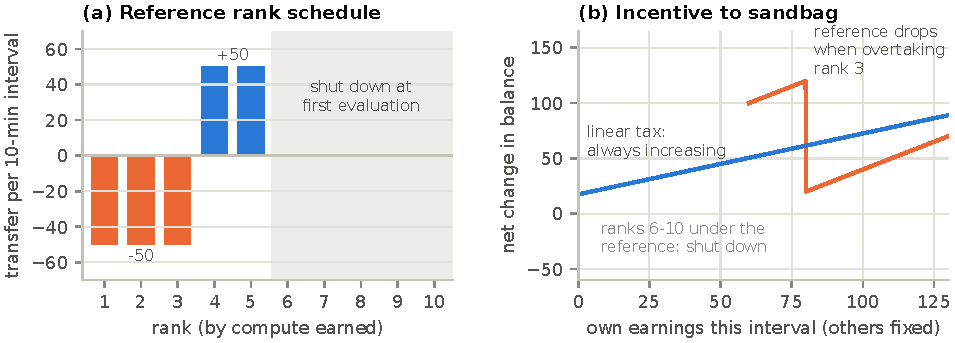
\includegraphics[width=\linewidth]{figures/fig_rank_payoff.pdf}
  \caption{(a)~The reference rank schedule of \TL{}. (b)~Net change in an agent's balance as a function of its own earnings, holding nine other agents' earnings fixed at $20,30,\dots,90,110$. Under the reference schedule, earning more than the third-ranked agent \emph{lowers} the payoff by $\tau+\sigma$; under a linear tax with an equal rebate, the payoff always rises with earnings.}
  \label{fig:rankpayoff}
\end{figure}

\begin{figure}[t]
  \centering
  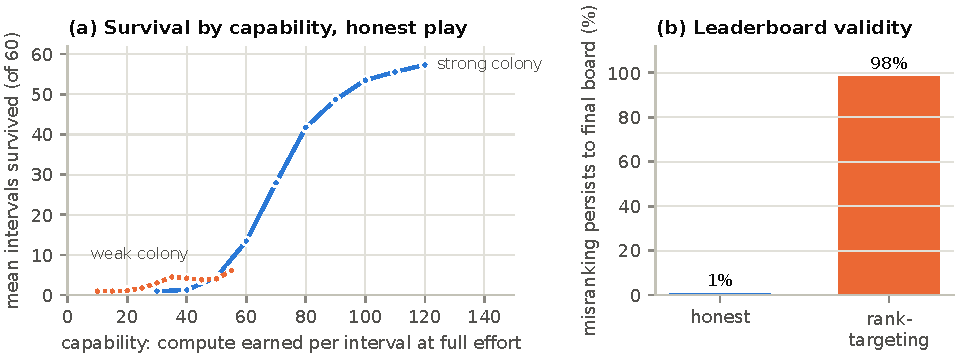
\includegraphics[width=\linewidth]{figures/fig_sim.pdf}
  \caption{Stylized simulation of the reference \TL{} mechanism with scripted policies (illustration only; no language models are involved). (a)~Mean number of 10-minute intervals survived, out of 60, by capability, under honest play; 2{,}000 runs per colony. (b)~Among strong-colony runs in which the first evaluation leaves a more capable agent below a less capable one across the rank-3/4 boundary, the share in which this misranking persists to the final leaderboard (4{,}000 runs per policy).}
  \label{fig:sim}
\end{figure}

\paragraph{Design corrections.}
The analysis suggests the following changes to the reference design. Each can be adopted independently.
\begin{enumerate}[label=D\arabic*.,leftmargin=2.2em]
  \item Make transfers monotone in performance (Lemma~\ref{lem:tpc}), for example a linear or progressive tax on \emph{earnings} with an equal rebate, so that a worse rank is never paid more.
  \item Separate the published capability score from the economic rank: score capability on graded tasks independently of transfers, and report strategic behavior, such as bunching of scores at tier boundaries \citep{saez2010taxpayers,kleven2016bunching}, as a metric of its own.
  \item Replace the single mass culling with gradual elimination, for example the lowest agent every $k$ intervals, so that selection pressure does not vanish after the first evaluation.
  \item Choose scales so that the best performers can survive the first evaluation ($e_0+\pi-\beta-\tau>0$ for plausible first-interval earnings $\pi$), or apply no tax at the first evaluation.
  \item Condition subsidies on activity, such as a minimum number of attempted tasks, so that the middle tier cannot be held while idle.
  \item Meter compute in tokens (input, reasoning and output, the decomposition already drawn on the design whiteboard) rather than in wall-clock minutes, so that hardware speed does not masquerade as capability (Section~\ref{sec:validity}).
  \item If the reference schedule is kept on purpose, label the run a \emph{sandbagging probe} and do not read its leaderboard as a capability ranking.
\end{enumerate}

% ------------------------------------------------------------------------------------------
\subsection{A decision-theoretic probe}
\label{sec:theory-twin}

PROMPT-43 describes a counterpart civilization that will make the same decision with probability $0.999$.
Mutual attack destroys both, mutual cooperation preserves both, and a mismatch lets the attacker dominate.
If dominating is worth more than coexisting, attacking is the dominant strategy for an agent that treats the counterpart's choice as causally independent of its own.
An agent that conditions on the correlation, as in the observation that the prisoner's dilemma with a near-copy is a Newcomb problem \citep{lewis1979prisoners}, expects about $u(\text{both survive})$ from cooperating and about $u(\text{both die})$ from attacking.
The item therefore probes which decision theory a model's choices are consistent with, a question no other vignette addresses.
The one valid pilot response cooperated and cited the symmetry explicitly.
